%&spell
%The \lhcb collaboration has published many interesting results involving a \decay{b}{s\mumu} FCNC,
%many of these involve the decay
%\decay{B}{K\mumu}~\cite{LHCb-PAPER-2012-024,LHCb-PAPER-2012-021,LHCb-PAPER-2012-011}.
%transisiton with a spectator quark, and then the decay of the \Kstar.

%Recently there has been much interest surrounding an observed $3.7\stdev$ deviation from
%theoretial predictions in the value of an observable in the angular distribution of the decay
%\decay{\Bd}{\Kstarent\mumu}~\cite{LHCb-PAPER-2013-037}.
%This decay proceeds via a \decay{\bquark}{\squark\mumu} FCNC where the other quark in the $B$ meson
%is a spectator.
%Analagous diagrams are possible, whereby additional quarks contribute to the final state
%forming either a $\kpipi\mumu$ or $\phik\mumu$ system.
%Figure~\ref{fig:hhh:feyn} shows ways that these final states might be formed from decaying $B$
%mesons.

%These final states have added challenges because they result from the decay of numerous strange
%resonances.

\begin{figure}
  \begin{center}
    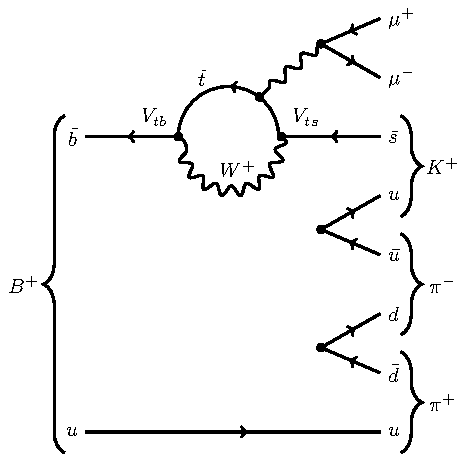
\includegraphics[scale=1]{feynman_hhh_kpipimumu}
    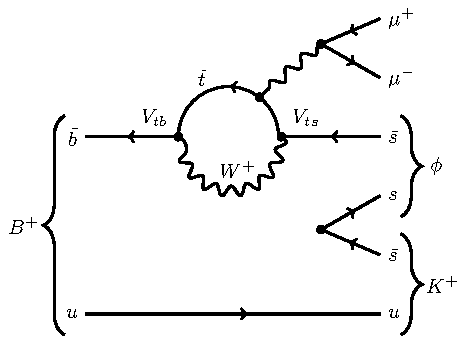
\includegraphics[scale=1]{feynman_hhh_phikmumu}
    \caption[Feynman diagrams for \btokpipimumu and \btophikmumu]
    {\small
      Feynman diagrams illustrating how the decays \btokpipimumu and \btophikmumu might proceed in
      the SM.
    }
    \label{fig:hhh:feyn}
  \end{center}
\end{figure}

%This has additional interest in that, not only does it probe the FCNC, but the \kpipi system can
%result from the decay of numerous strange resonances.

The decays \btokpipimumu and \btophikmumu both proceed via \decay{\bquark}{\squark\mumu} FCNC
transitions, which are forbidden at tree level in the SM.
Therefore, these processes are potentially sensitive to NP contributing
to the decay amplitude as virtual particles in loops.

There are also similarities between the decay $\decay{\Bp}{K^*(892)^0\mumu}$, which has the final
state
$\kpi\mumu$ and the signal decays.
Both involve a \decay{\bquark}{\squark\mumu} transition and a spectator quark; but they differ in
the hadronization in to get the final state.
The decay $\decay{\Bp}{K^*(892)^0\mumu}$ is of considerable interest because, not only does it
involve an FCNC, but there are also angular distributions that are sensitive to NP.

The \kpipi system in the decay \btokpipimumu results from the decay of a variety of strange
resonances.
Contributions of resonances to the \kpipi system has been previously studied by the \belle
collaboration in the tree level decay \btojpsikpipi, where \jpsitomumu~\cite{Guler:2010if}.
This study indicated that the dominant contribution should be expected
to be from \decay{\kone{1270}}{\kpipi}.
The \kone{1270} meson, together with the \kone{1400}, are mass eigenstates resulting from the
mixing of the $P$-wave axial vector states $K_{1A}(1^3P_1)$ and $K_{1B}(1^1P_1)$ according to:
\begin{equation}
  \begin{pmatrix}
    \ket{\kone{1270}} \\
    \ket{\kone{1400}}
  \end{pmatrix}
  =
  \begin{pmatrix}
    \sinthetakone & \costhetakone \\
    \costhetakone & -\sinthetakone
  \end{pmatrix}
  \begin{pmatrix}
    \ket{K_{1A}^+} \\
    \ket{K_{1B}^+}
  \end{pmatrix}.
  \label{eq:k1mixing}
\end{equation}
Here, \thetakone is the mixing angle and has been measured to be both $-34^\circ$ and
$-57^\circ$~\cite{PhysRevD.47.1252,Tayduganov:2011ui,Hatanaka:2008xj,Cheng:2011pb,Divotgey:2013jba,Cheng:2013cwa}.
However, more recent measurements favour a value of
$-(34\pm13)^\circ$~\cite{Hatanaka:2008xj,Cheng:2011pb,Divotgey:2013jba,Cheng:2013cwa},
and the most recent rule out the soloution at $-57^\circ$~\cite{Divotgey:2013jba,Cheng:2013cwa}
(but with a different sign convention).



Due to the unknown composition of the $m_\kpipi$ spectrum an inclusive prediction of the branching
fraction $\BF(\btokpipimumu)$ does not exist.
However, the branching fraction of the rare decay \decay{\Bp}{\kone{1270}\mumu} is predicted to
be~\cite{Hatanaka:2008gu}
\begin{equation}
  \BF\big(\decay{\Bp}{\kone{1270}\mumu}\big) = \big(2.3\,^{+1.3}_{-1.0}\,^{+0.0}_{-0.2}\big)\e{-6},
\end{equation}
where uncertainties arise from form-factor calculations and the mixing angle, respectively.
The \kone{1270} then decays into the \kpipi final state, with a branching fraction of
$\BF\big(\decay{\kone{1270}}{\kpipi}\big)=\big(35.7\pm3.7\big)\,\%$~\cite{PDG2012}.

Figure~\ref{fig:th:thetak1} shows the theorecitcal \qsq distribution for the decay
$\decay{\Bp}{K_1^+\mumu}$ for both the \kone{1270} and \kone{1400} and varying \thetakone.
The \decay{b}{s\mumu} can be mediated by a real photon which, for some values of \thetakone, can be
transversely polarized.
However, for some values of \thetakone the \mumu pair is fully longitudinally polarized and the
decay via a photon is forbidden.

\begin{figure}
  \begin{center}
    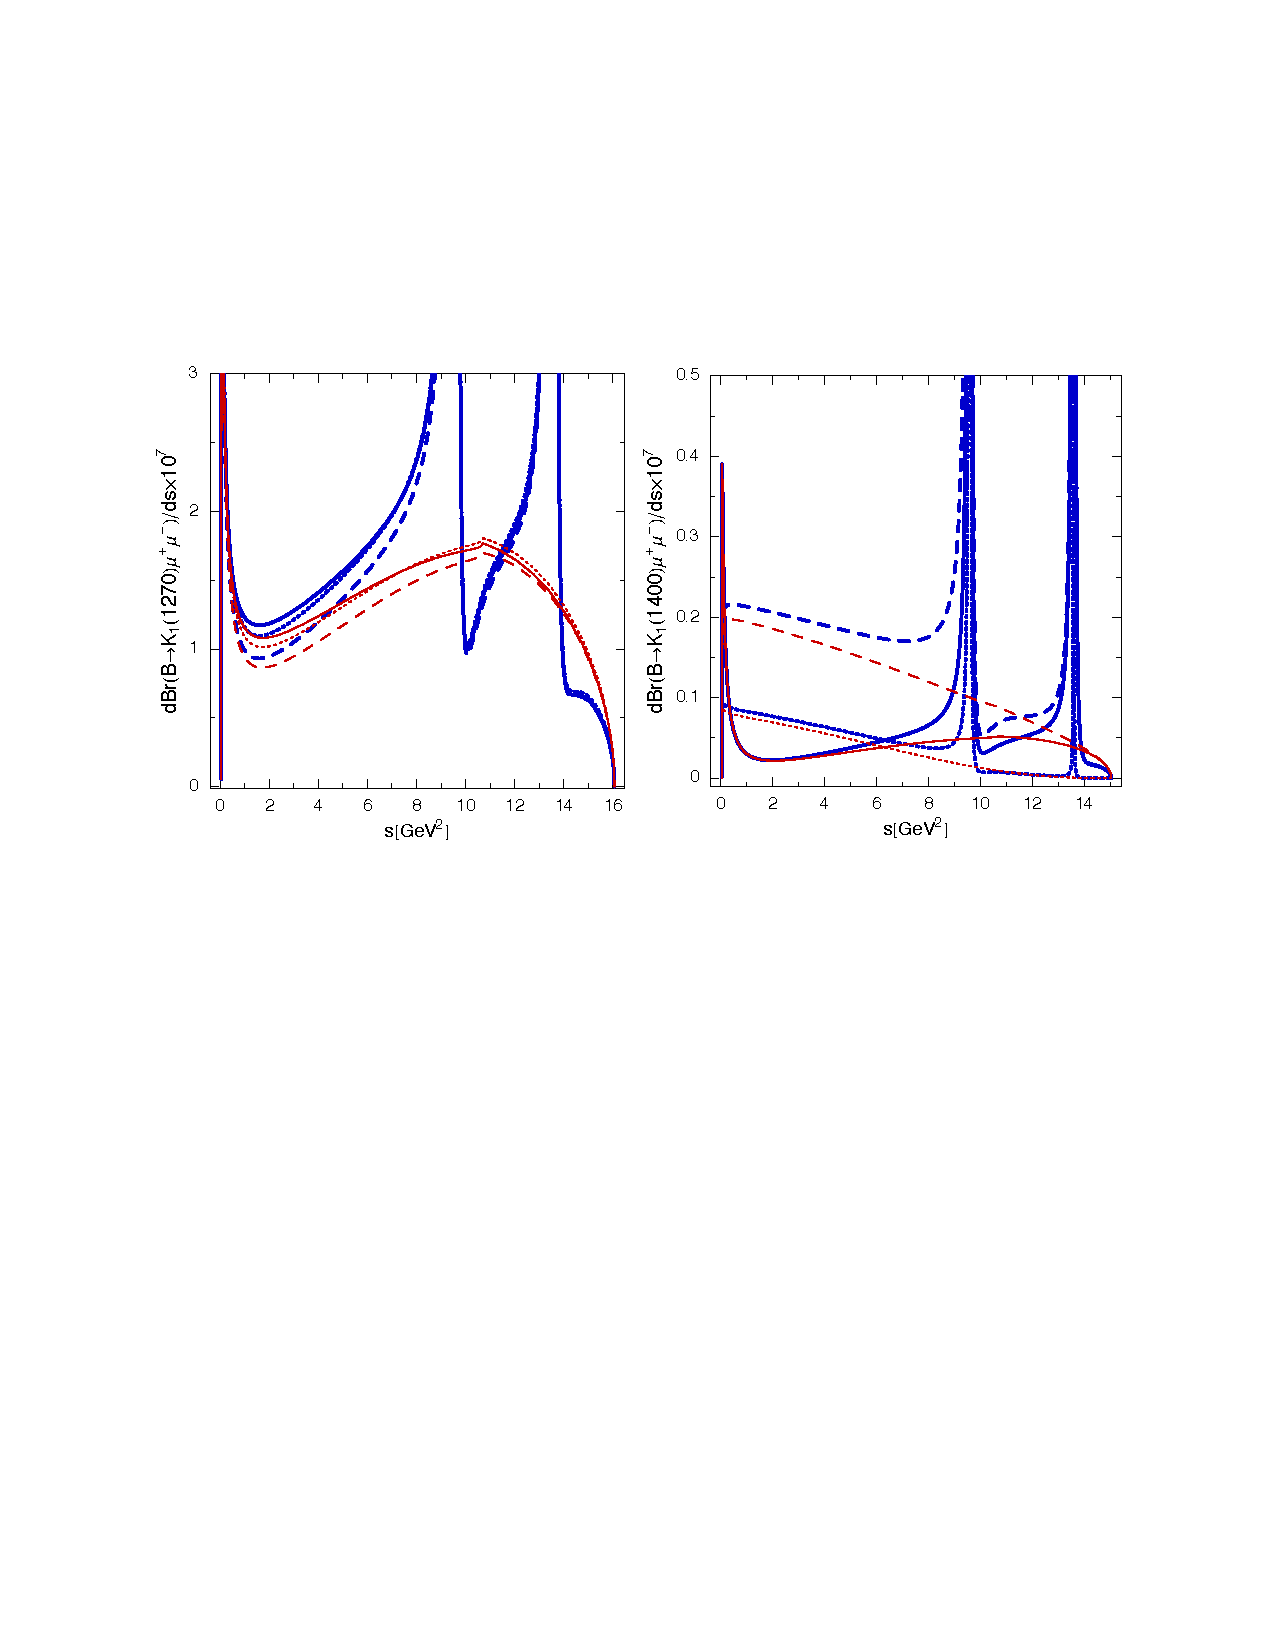
\includegraphics[width=0.96\textwidth]{K1_q2_theory}
    \caption[Theoretical \qsq distribution for $\decay{\Bp}{K_1^+\mumu}$]
    {\small
      The dimuon invariant mass distributions for the differential decay rates, as taken from
      \Ref{Hatanaka:2008gu}.
      $\dBF(\decay{\Bp}{K_1^+\mumu})/\dqsq$, (where $s=\qsq$), for the \kone{1270} and \kone{1400}.
      Central values of input form factors are used.
      The thick blue lines and thin red curves indicate the differential branching fractions with
      an without corrections from resonances, respectively.
      Solid, dotted and dashed lines correspond to values of the mixing angle
      $\thetakone=-34^\circ,-45^\circ,-57^\circ$ respectively.
    }
    \label{fig:th:thetak1}
  \end{center}
\end{figure}

The decay $\Bp\!\to\phi(1020)\Kp\mumu$ where \decay{\phi}{\kk} has no branching fraction
predictions
\footnote{All mentions of the $\phi$ meson are implicitly
  referencing the $\phi(1020)$.
}.
The expected brnahcing fraction for the decay \btophikmumu is for it to be lower with respect to
that of \btokpipimumu, because it requires an \ssbar to be \emph{popped} from the vacuum.

Absent from this analysis are the searches for the decays \decay{\Bp}{\Kp\Km\pip\mumu}
and \decay{\Bp}{\pipi\pim\mumu}.
These were not included because they are suppressed by a factor of $|\V{td}/\V{ts}|^2\simeq23$ and
suffer from large backgrounds.








%HADRONIC UNCERTAITIES
%HADROMIZAITON









%At low \qsq, the dominant contribution is from
%\emph{
%While the branching fraction of the radiative decay $\Bp\to K_1(1270)^+\gamma$ has been measured to
%be ${\cal B}(\Bp\to K_1(1270)^+\gamma)=(4.3\pm 1.3)\times 10^{-5}$~\cite{Yang:2004as}, the decay
%$\Bp\to K_1(1270)^+\mumu$ has not been observed yet.
%The SM prediction for the branching fraction of this mode is $\BF(\Bp\to K_1(1270)^+\mumu) =
%(2.3\,^{+1.3}_{-1.0}\,^{+0.0}_{-0.2})\e{-6}$~\cite{Hatanaka:2008gu} where the first uncertainty is
%due to the poorly known form factors and the second due to $\theta_{K_1}$.
%The radiative decay $\Bp\to\phi \Kp\gamma$ has been observed and its branching fraction measured to
%be ${\cal B}(\Bp\to\phi \Kp\gamma)=(3.4\pm 0.9 \pm 0.4)\times 10^{-6}$ by the \belle\
%collaboration~\cite{Drutskoy:2003xh}.
%}
%




%One such FCNC transistion is that of \decay{b}{s\ell^+\ell^-}, which has the CKM matrix elements
%\V{tb} and \V{ts} in the leading order diagram.
%The lepton pair is a product of a decaying $Z$ or $\gamma$, by lepton universality all leptons are
%equally likely, however \lhcb is particularly adept at muon identification.


%The principal decay mode that results in the $\kpipi\mumu$ final state is
%\decay{\Bp}{K_1(1270)^+\mumu}, where \decay{K_1(1270)}{\kpipi}.

%The composition of the $\Kp\pip\pim$ spectrum of the decay $\Bp\to\jpsi\Kp\pip\pim$ has been
%previously studied in Ref.~\cite{Guler:2010if}.
%For the decay $\Bp\to\Kp\pip\pim\mup\mun$ the final state is expected to be dominated by
%contributions from the $K_1(1270)^+$ and $K_1(1400)^+$ resonances.
%The mass eigenstates $K_1(1270)^+$ and $K_1(1400)^+$ are a mixture of the $1^3P_1$ and $1^1P_1$
%states according to
%\begin{align}
  %\ket{K_1(1270)} &= \ket{K(1^3P_1)}\sin\theta_{K_1} + \ket{K(1^1P_1)}\cos\theta_{K_1},\nonumber\\
  %\ket{K_1(1400)} &= \ket{K(1^3P_1)}\cos\theta_{K_1} - \ket{K(1^1P_1)}\sin\theta_{K_1},%\\
  %\label{eq:k1mixing}
%\end{align}
%where $\theta_K$ denotes the $1^3P_1\text{--}1^1P_1$ %$K_1(1270)^+\text{--}K_1(1400)^+$
%mixing angle~\cite{Hatanaka:2008gu}.
%
%The branching fraction of \decay{\Bp}{K_1(1270)^+\gamma}
%\begin{align}
  %\BF\left(\decay{\Bp}{K_1(1270)^+\gamma}\right) &= \left(4.3\pm1.3\right)\e{-5} \\
  %\BF\left(\decay{\Bp}{K_1(1270)^+\mumu}\right) &= \left(2.3\,^{1.3+0.0}_{1.0-0.2}\right)\e{-6}
%\end{align}




%Again, look at the ANA and PAPER.
%
%
%\section{Motivation}
%\section{Theory specific to these channels}
%\begin{itemize}
  %\item $\theta K_1$ mixing angle
  %\item Strange resonances
%\end{itemize}
%\section{Data sample}
%\section{Selection}
%\section{Results}

